\newcommand{\orgmode}{\texttt{org-mode}}
\newcommand{\Makefile}{\mintinline{shell}{Makefile}}
\newcommand{\context}{\mintinline{shell}{context}}
\newcommand{\CC}{C\nolinebreak\hspace{-.05em}\raisebox{.4ex}{\tiny\bf +}\nolinebreak\hspace{-.10em}\raisebox{.4ex}{\tiny\bf +}}
\def\CC{{C\nolinebreak[4]\hspace{-.05em}\raisebox{.4ex}{\tiny\bf ++}}}

\section{Introduction}


The ultimate goal of \ac{QMCkl} is to provide a high-performance
implementation of the main kernels of \ac{QMC}. In this particular
\ac{WP}, we focus on the definition of the \ac{API}, the tests,
and on a \emph{pedagogical} presentation of the algorithms.  We expect
the \ac{HPC} experts to use this repository as a reference for re-writing
optimized versions of the functions described in this library, using
the same \ac{API}.

The documentation of the current status of the library is available
at \url{https://trex-coe.github.io/qmckl}, and the source code is
available on the GitHub repository at \url{https://github.com/trex-coe/qmckl}.


\subsection{Literate programming}

In a traditional code, most of the lines of source files are code,
scripts, {\Makefile}s, and only a few lines are comments explaining
parts of the code that are non-trivial to understand. The
documentation of the program is usually written in a separate
directory, and is often outdated with respect to the current version
of the code.

Literate programming\cite{knuth_1992} is a different approach to
programming, where the program is considered as a publishable-quality
document. Most of the lines of the source files are text,
mathematical formulas, tables, figures, \textit{etc}, and the lines of
code are just the translation in a computer language of the ideas
and algorithms expressed in the text. More importantly, the ``document'' is
structured like a text document with sections, subsections, a bibliography, and a table of contents. The place where pieces of code
appear are the places where they should belong for the reader to
understand the logic of the program, not the places where the compiler
expects to find them. Both the publishable-quality document and the
binary executable are produced from the same source files. 

Literate programming is particularly well adapted in this context, as
the central part of this project is the documentation of an
\ac{API}. The implementation of the algorithms is just an expression
of the algorithms in a language that can be compiled, so that the
correctness of the algorithms can be tested.

We have chosen to write the source files in {\orgmode}
format\cite{schulte_2012,orgmode}, as any text editor can be used to
edit {\orgmode} files. To produce the documentation, there exists
multiple possibilities to convert {\orgmode} files into different
formats such as \ac{HTML} or \ac{PDF}. The source code is easily
extracted from the {\orgmode} files invoking the Emacs text editor
from the command-line in the {\Makefile}, and then the produced files
are compiled as usual.  Moreover, within the Emacs text editor the
source code blocks can be executed interactively, as in Jupyter
notebooks\cite{Kluyver_2016}, but with the advantage that multiple
languages can be used in the same notebook.

\subsection{Algorithms}

Reducing the scaling of an algorithm usually implies also reducing its
arithmetic complexity (number of flops per byte). For small
sizes, \(\mathcal{O}(N^3)\) and \(\mathcal{O}(N^2)\) algorithms are
often better adapted than linear scaling algorithms. Indeed, the
reduction of the number of flops does not necessarily compensate the
high efficiency of BLAS3 implementations.
As \ac{QMCkl} is a general purpose library, multiple algorithms will
be implemented adapted to different ranges of sizes.

\subsection{Dependencies}

Dependencies are critical: if a user is not able to install the
required dependencies, the user is not going to be able to use our
library. So the list of
external dependencies should be kept as small as possible. 
External libraries should be used \emph{only} if their use is
strongly justified, and if we are sure that the users will be able to
have access to them.

The dependencies needed to use pre-compiled versions of the library
are \ac{BLAS} and \ac{LAPACK}.

The dependencies needed to compile the code are
a C and a Fortran compiler, GNU make, \ac{BLAS} and \ac{LAPACK}, and
$\mu$nit\cite{munit} for building the unit tests.

The dependencies needed to create the \ac{HTML} documentation are
Emacs~26 and the package Emacs-htmlize.

\subsection{Packaging}

We intend to use the GNU build system, Autotools,\cite{autotools} for
configuration and installation scripts.
Although there exists more modern build tools, we have chosen a
solution that will be easy for the end user, and which is one of the
most reliable in terms of portability among different architectures.

In the future, we plan to provide \texttt{.deb} and \texttt{.rpm}
packages for the most common Linux distributions, as well as a package
for the Spack package manager\cite{spack}.


\subsection{Continuous integration}

Continuous integration has been setup on the GitHub platform. Upon
receiving a pull request, the repository is automatically cloned on a virtual machine. The source code is then extracted from the {\orgmode}
files and the library is compiled. Then the unit tests are compiled
and linked together with the library. If all the tests pass, the
pull request is considered valid, and can be merged.

When the code is updated, the documentation is automatically built and
the server hosting the documentation is updated, such that the web
site containing the documentation is always synchronized with the
latest version of the master branch of the GitHub repository.


\section{Source code}

\subsection{Choice of the programming language}

Most of the codes of the \ac{TREX} \ac{CoE} are written in Fortran
with some scripts in Bash and Python. Outside of the
\ac{CoE}, Fortran is also important (Casino, Amolqc). Other
important languages used by the community are C and {\CC} (QMCPack,
QWalk). Python is very popular for prototyping, and Julia is gaining
in popularity\cite{poole_2020}. The library we design should be
compatible with at least all of these languages. A simple solution is
to provide a C-compatible \ac{API} since all these languages have a
\ac{FFI} for calling functions written in C, especially for
interacting with the operating system.

High-performance versions of the \ac{QMCkl}, with the same \ac{API},
will be rewritten in \ac{WP}3 by the experts in \ac{HPC}. These
optimized libraries will be tuned for specific architectures, among
which we can cite x86 based processors and \ac{GPU} accelerators.
Nowadays, there exists very efficient and popular software tools to
take advantage of low-level features of the processor\cite{pohl_2016}
(vectorization intrinsics) and of \acp{GPU} accelerators (SYCL\cite{SYCL},
OneAPI, Kokkos\cite{kokkos}) for {\CC} developers. So it is very likely
that some optimized implementations will be written in {\CC}, and this
is agreement with our choice to make the \ac{API} C-compatible.

Fortran is one of the most common languages used by the community, and
is simple enough to make the algorithms readable both by experts in
\ac{QMC}, and experts in \ac{HPC}. Hence we propose in this
pedagogical implementation of \ac{QMCkl} to use Fortran to express the
QMC algorithms, but we expose them through the \ac{API} as if they
were written in C using the \mintinline{fortran}{iso_c_binding} \ac{FFI}.

To avoid collisions in the names of the compiled files, the names of
the Fortran source files end with \mintinline{shell}{_f.f90}, and Fortran
interface files end with \mintinline{shell}{_fh.f90}.
The names of the functions defined in Fortran should be the
same as those exposed in the \ac{API} suffixed by \mintinline{shell}{_f}.

When the library is built, a single shared library is produced
(\mintinline{shell}{libqmckl.so}). All the function prototypes are given in a single C
header file \mintinline{shell}{qmckl.h}, and a Fortran interface to the library
is provided via a module containing only interfaces to the C functions
(\mintinline{shell}{qmckl_f.f90}).

\subsection{License}

The library is licensed under the open-source 3-clause BSD license to facilitate
its adoption in all quantum chemistry software, commercial or not.


\section{Design of the library}

The proposed \ac{API} should allow the library to deal with memory
transfers between CPU and accelerators, and to use dynamically
different levels of floating-point precision.  We chose a
multi-layered design with low-level and high-level functions (see
below).

\subsection{Naming conventions}

To avoid namespace collisions, we use \mintinline{C}{qmckl_} as a prefix for
all exported functions and variables.  All exported header files
should have a file name prefixed with \mintinline{shell}{qmckl_}.

For instance, if the name of the {\orgmode} file is
\mintinline{shell}{xxx.org}, the name of the produced C files should
be \mintinline{shell}{xxx.c} and \mintinline{shell}{xxx.h} and the
name of the produced Fortran file should be
\mintinline{shell}{xxx.f90}

Arrays are in uppercase and scalars are in lowercase.

In the  names of  the variables and  functions, only the singular
form is allowed.

\subsection{Application programming interface}

In the C language, the number of bits used by the basic integer types
(\mintinline{C}{int}, \mintinline{C}{long int}, \textit{etc}) can
change from one architecture to the other. To circumvent this
problem, we choose to use the integer types defined in
\mintinline{C}{<stdint.h>} where the number of bits used to represent
integers are fixed.

To ensure that the library will be easily usable in \emph{any} other
language than C, we restrict the data types in the interfaces to the
following:
\begin{itemize}
\item 32-bit and 64-bit integers, scalars and and arrays
  (\mintinline{C}{int32_t} and \mintinline{C}{int64_t})
\item 32-bit and 64-bit floats, scalars and and arrays
  (\mintinline{C}{float} and \mintinline{C}{double})
\item Pointers are always casted into 64-bit integers, even on legacy 32-bit architectures
\item ASCII strings are represented as a pointers to character arrays
  and terminated by a zero character (C convention).
\item Complex numbers can be represented by an array of 2 floats.
\item Boolean variables are stored as integers, \mintinline{C}{1} for
\mintinline{C}{true} and \mintinline{C}{0} for \mintinline{C}{false}
\item Floating point variables should be by default
\mintinline{C}{double}, unless explicitly mentioned
\item integers used for counting should always be \mintinline{C}{int64_t}
\end{itemize}

To facilitate the  use in other languages than C, we plan to provide 
bindings for other languages.


\subsubsection{Global state}

Global variables should  be avoided in the library,  because it is
possible that one  single program needs to  use multiple instances
of the library, or to use the library in a multi-threaded context.
To solve this  problem we propose to use a pointer
to a {\context}  variable,  built   by  the  library   with  the
\mintinline{C}{qmckl_context_create} function. The
{\context} contains the global state of the library, and is used as
the first argument of most \ac{QMCkl} functions.

The internal structure of the {\context}  is not specified, to give a
maximum of  freedom to  the different  implementations.  Modifying
the  state   is  done   by  setter   and  getter functions,   prefixed  by
\mintinline{C}{qmckl_context_set_}  an
\mintinline{C}{qmckl_context_get_}.
When a {\context} variable is modified by a setter, a copy of the old
data structure is made and updated, and the pointer to the new data
structure is returned, such that the old contexts can still be
accessed in case they are already involved in running computations by
other threads. It is also possible to modify the state in an mutable
fashion, using the \mintinline{C}{qmckl_context_update_} functions,
although it is not recommended as the default practice.
The {\context} and its old versions can be destroyed with
\mintinline{C}{qmckl_context_destroy}.


\subsubsection{Low-level functions}

Low-level functions are very simple functions which are leaves of
the function call tree (they don't call any other \ac{QMCkl} function).
These  functions   are   \emph{pure} (i.e. without side effects), and
unaware of the \ac{QMCkl} {\context}. They are not allowed to
allocate/deallocate memory, and if they need temporary memory it
should be provided in input. This will prevent a degradation of
performance due to unnecessary repeated memory allocations and
deallocations hot spots of the programs.


\subsubsection{High-level functions}

High-level functions  are higher in the function  call tree.
They  are  able  to  choose which  lower-level  function  to  call
depending on the required precision, and to do the corresponding type
conversions. They are also able to choose between different algorithms
(sparse or dense for example), according to parameters defined in the
{\context}.  These functions are also responsible for allocating
temporary storage, to optimize the use of accelerators.

The high-level functions should be pure, unless if it is
justified. If any, all the side effects should be made in the
\texttt{context} variable.

\subsubsection{Numerical precision}

The number of bits of precision  required for a function should be
given as an input of low-level computational functions. This input
will be used to define the values of the different thresholds that
might be used to avoid computing unnecessary numerical
noise. High-level functions will use the precision specified in the
\texttt{context} variable.


\section{Codesign}
\label{sec:codesign}

Research codes are developed over a long period of time by multiple
researchers, Ph.D students and post-docs. The professional evaluation
of these people is based on their scientific production and not on the
quality of the software they write, so code quality and refactoring is
often left in the low-priority task queue. As a consequence, research
codes often depend on some choices made at an immature stage of the
program, and solutions to bypass the wrong choices make the code
complicated to understand for external programmers, especially if they
are not familiar with the domain.

\subsection{Kernel extraction}

The strategy we have chosen to extract the kernels of the codes is to
first discuss among the developers of \ac{QMC} codes to understand how they have
implemented each particular kernel. Once the developers have agreed on
which algorithm is best, they first formulate the algorithm in terms
of mathematical expressions in a {\LaTeX} file, and they create a prototype application 
(the \emph{mini-application}) implementing \emph{only} the kernel of
interest. This mini-application can be easily compiled and executed,
and is considered valid when it reproduces exactly the values obtained
with the kernel present in the original \ac{QMC} code.

The mini-application is then thoroughly modified together with the
\ac{HPC} experts involved in \ac{WP}3 until the optimal data
structures and algorithms are determined. This step is crucial to
facilitate the access to performance in the \ac{HPC} versions of the
library that will be developed in \ac{WP}3.  Once the \ac{QMC} and
\ac{HPC} specialists have agreed on the data structures, the kernel is
ready to be implemented in the
library.


\subsection{A concrete example}

The first kernel we have been working on is the three-body component of
the Jastrow factor, which is one of the potential bottlenecks of
extreme-scale calculations that will run on exascale machines.
In the CHAMP program, it is expressed as

\newcommand{\Jeen}{J_{\text{een}}}
\newcommand{\Nel}{N_{\text{elec}}}
\newcommand{\Nat}{N_{\text{nucl}}}
\newcommand{\Nord}{N_{\text{nord}}}
\newcommand{\lmax}{p-k-2\delta_{k,0}}
\newcommand{\br}{\mathbf{r}}
\newcommand{\bR}{\mathbf{R}}
\[
  \Jeen (\br,\bR) = \sum_{\alpha=1}^{\Nat} \sum_{i=1}^{\Nel} \sum_{j=1}^{i-1}
\sum_{p=2}^{\Nord} \sum_{k=0}^{p-1}
\sum_{l=0}^{\lmax} c_{lkp\alpha}
\left( {r}_{ij} \right)^k
\left[ \left( {R}_{i\alpha} \right)^l + \left( {R}_{j\alpha} \right)^l \right]
\left( {R}_{i\,\alpha} \, {R}_{j\alpha} \right)^{(p-k-l)/2} 
\]
where
$\Nel$ is the number of electrons, 
$\Nat$ is the number of nuclei,
$\Nord$ is the maximum order of the polynomial, 
$\br$ contains rescaled electron-electron distances, 
$\bR$ contains rescaled electron-nucleus distances,
and $c_{lkp\alpha}$ are the variational parameters which are non-zero
only when $p-k-l$ is even.

For \ac{QMC} simulations, the first and second derivatives of $\Jeen$ with
respect to the electron coordinates are also required. To optimize the
parameters, the derivative with respect to $c_{lkp\alpha}$
should also be available, and in the context of molecular dynamics or
geometry optimization the first derivatives with respect to $\bR$ are
also required. To compute these derivatives, multiple intermediates
will be common and we need to identify them such that the same
intermediates can be reused for several derivatives.

We have written a mini-application to implement the three-body component
of the Jastrow factor, as well as the first and second derivative with
respect to electron coordinates. This mini-application, available on
GitHub\footnote{\url{https://github.com/trex-coe/irpjast}} has allowed us to
rewrite the expressions in a way allowing us to take advantage of BLAS3
matrix multiplications. The formula is now expressed in terms of
rank-3 and rank-4 tensors
\newcommand{\tr}{\, \bar{\mathtt{r}}}
\newcommand{\tR}{\, \bar{\mathtt{R}}}
\newcommand{\tP}{\, \bar{\mathtt{P}}}
\[
  \Jeen(\br,\bR) = 
  \sum_{p=2}^{\Nord}\sum_{k=0}^{p-1}
  \sum_{l=0}^{\lmax} 
    \sum_{\alpha=1}^{\Nat}
    c_{lkp\alpha}
    \sum_{i=1}^{\Nel}
    {\tR}_{i,\alpha,(p-k-l)/2}\,
  {\tP}_{i,\alpha,k,(p-k+l)/2}
  \]
with 
  \[
  {\tP}_{i, \alpha, k, l} = \sum_{j=1}^{\Nel} {\tr}_{i,j,k}\,{\tR}_{j,\alpha,l}.
  \]
  
Similarly, the gradient with respect to electron coordinates and the
Laplacian require an additional intermediate array and reuses ${\tP}$. As
the gradient ($\nabla_{i}$) and the Laplacian ($\Delta_i$) have a
large part of their expression in common, the $3\Nel$ components of
the gradient and the $\Nel$ components of the Laplacian are stored in
the same array, adding an extra index $m=(1,2,3)$ for $\nabla_x,
\nabla_y,\nabla_z$
and $m=4$ for $\Delta$.

\newcommand{\tg}{\, \bar{\mathtt{g}}}
\newcommand{\tG}{\, \bar{\mathtt{G}}}
\newcommand{\tQ}{\, \bar{\mathtt{Q}}}

\begin{eqnarray*}
  \nabla_{im} \Jeen(\br,\bR) & = &
  \sum_{p=2}^{\Nord}\sum_{k=0}^{p-1}
  \sum_{l=0}^{\lmax} 
    \sum_{\alpha=1}^{\Nat}
    c_{lkp\alpha}
    \sum_{i=1}^{\Nel} 
     {\tG}_{i,m,\alpha,(p-k-l)/2} {\tP}_{i,\alpha,k,(p-k+l)/2} +  \\
&&   {\tG}_{i,m,\alpha,(p-k+l)/2} {\tP}_{i,\alpha,k,(p-k-l)/2} + 
     {\tR}_{i,\alpha,(p-k-l)/2} {\tQ}_{i,m,\alpha,k,(p-k+l)/2} + \\
&&   {\tR}_{i,\alpha,(p-k+l)/2} {\tQ}_{i,m,\alpha,k,(p-k-l)/2} + 
    \delta_{m,4} \big( \\
&&     {\tG}_{i,1,\alpha,(p-k+l)/2} {\tQ}_{i,1,\alpha,k,(p-k-l)/2} +
       {\tG}_{i,2,\alpha,(p-k+l)/2} {\tQ}_{i,2,\alpha,k,(p-k-l)/2} + \\
&&     {\tG}_{i,3,\alpha,(p-k+l)/2} {\tQ}_{i,3,\alpha,k,(p-k-l)/2} +
       {\tG}_{i,1,\alpha,(p-k-l)/2} {\tQ}_{i,1,\alpha,k,(p-k+l)/2} + \\
&&     {\tG}_{i,2,\alpha,(p-k-l)/2} {\tQ}_{i,2,\alpha,k,(p-k+l)/2} + 
       {\tG}_{i,3,\alpha,(p-k-l)/2} {\tQ}_{i,3,\alpha,k,(p-k+l)/2} \big)
\end{eqnarray*}
with 
\[
  {\tG}_{i, m, \alpha, l}  =  \frac{\partial \left( {R}_{i\alpha} \right)^l}
                             {\partial r_i},  \phantom{ space }
  {\tg}_{i, m, j, k}  =  \frac{\partial \left( {r}_{ij} \right)^k}
                             {\partial r_i}, \phantom{ space }
                             \text{ and } 
  {\tQ}_{i, m, \alpha, k, l}  =  \sum_{j=1}^{\Nel}
                            {\tg}_{i,m,j,k}\,{\tR}_{j,\alpha,l} 
\]
  
\begin{figure}[t]
  \begin{center}
  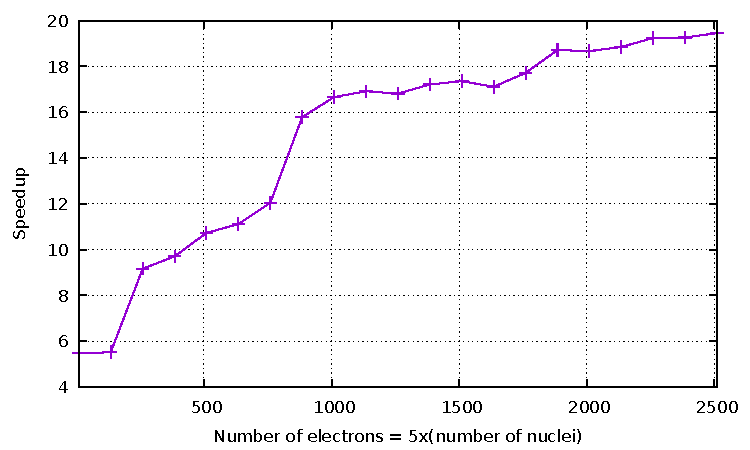
\includegraphics[width=0.75\textwidth]{speedup.pdf}
  \end{center}
  \caption{\label{fig:speedup}Speedup obtained after the re-expression of the three-body
    Jastrow factor.}
\end{figure}

This rewriting allowed us to move the computationally intensive part in
$\mathcal{O}(\Nat{\Nel}^2)$, i.e. the construction of the intermediate
tensors, into a BLAS3 matrix multiplication, the remaining part being
in $\mathcal{O}(\Nat \Nel)$.

The performance of the computation of the value, gradient and Laplacian of
the three-body Jastrow factor was measured on an Intel(R) Xeon(R) Gold
6130 processor, and the code was compiled with the Intel Fortran
compiler version 2021.1 with options
\mintinline{bash}{-O3 -xCORE-AVX512 -g -mkl=sequential -qopt-zmm-usage=high}.
The speedup with respect to the unoptimized kernel is presented in
figure~\ref{fig:speedup}, and reaches a factor of $19\times$ for the
largest system sizes. Performance analyzis of the mini-application
showed that at this stage we have reached 80\% of the single core peak
performance of the CPU core for this kernel. Profiling with MAQAO
confirmed a the high quality of the code produced by our mini-application.

The same strategy of kernel extraction of the codes and rewriting
will be applied to all other possible computational bottlenecks of QMC
simulations, and then the kernels will be ready to be implemented in
the library.




\appendix
\section{Appendix: Documentation of the API}

In this section, we include as an example part of the documentation of
the library which is automatically generated from the {\orgmode}
files, in the current status. The rest of the documentation can be
found on the web site of the library\footnote{\url{https://trex-coe.github.io/qmckl}}.
Please, keep in mind that the library is still at an early development
stage. In the first six months, most of the effort was made on
preparing solid bases for the development of
the library, more related to system programming than scientific
programming (the context variable, memory allocation, conventions,
Makefiles, generation of the documentation, \textit{etc}). The actual
implementation of the kernels is just starting.


\clearpage

\section*{Context}

The context variable is a handle for the state of the library,
and is stored in a data structure which can't be seen outside of
the library.  To simplify compatibility with other languages, the
pointer to the internal data structure is converted into a 64-bit
signed integer, defined in the \texttt{qmckl\_context} type.
A value of \texttt{QMCKL\_NULL\_CONTEXT} for the context is equivalent to a
\texttt{NULL} pointer.

\begin{minted}[frame=lines,fontsize=\scriptsize,linenos]{c}
typedef int64_t qmckl_context ;
#define QMCKL_NULL_CONTEXT (qmckl_context) 0
\end{minted}

\subsection{Context handling}
\label{sec:org502090e}

The context appears as an immutable data structure: modifying a
context returns a new context with the modifications.  Therefore, it
is necessary to store a pointer to the old version of context so
that it can be freed when necessary.
Note that we also provide a possibility to mutate the context, but
this should be done with caution, only when it is justified.

By convention, in this file \texttt{context} is a \texttt{qmckl\_context} variable
and \texttt{ctx} is a \texttt{qmckl\_context\_struct*} pointer.

\subsubsection{Data structure}
\label{sec:orgca6cd07}

The main data structure contains pointers to other data structures,
containing the data specific to each given domain, such that the
modified contexts don't need to duplicate the data but only the
pointers.

\begin{minted}[frame=lines,fontsize=\scriptsize,linenos]{c}
typedef struct qmckl_context_struct {

  /* Pointer to the previous context, before modification */
  struct qmckl_context_struct * prev;

  /* Molecular system */
  qmckl_ao_basis_struct    * ao_basis;

  /* To be implemented:
  qmckl_nucleus_struct     * nucleus;
  qmckl_electron_struct    * electron;
  qmckl_mo_struct          * mo;
  qmckl_determinant_struct * det;
  */

  /* Numerical precision */
  qmckl_precision_struct   * fp;

  /* Error handling */
  qmckl_error_struct       * error;

  /* Memory allocation */
  qmckl_memory_struct      * alloc;

  /* Thread lock */
  int                        lock_count;
  pthread_mutex_t            mutex;

  /* Validity checking */
  uint32_t                   tag;

} qmckl_context_struct;
\end{minted}


A tag is used internally to check if the memory domain pointed
by a pointer is a valid context. This allows to check that even if
the pointer associated with a context is non-null, we can still
verify that it points to the expected data structure.

\begin{minted}[frame=lines,fontsize=\scriptsize,linenos]{c}
#define VALID_TAG   0xBEEFFACE
#define INVALID_TAG 0xDEADBEEF
\end{minted}

The \texttt{qmckl\_context\_check} function checks if the domain pointed by
the pointer is a valid context. It returns the input \texttt{qmckl\_context}
if the context is valid, \texttt{QMCKL\_NULL\_CONTEXT} otherwise.

\begin{minted}[frame=lines,fontsize=\scriptsize,linenos]{c}
qmckl_context qmckl_context_check(const qmckl_context context) ;
\end{minted}

\begin{minted}[frame=lines,fontsize=\scriptsize,linenos]{c}
qmckl_context qmckl_context_check(const qmckl_context context) {

  if (context == QMCKL_NULL_CONTEXT)
    return QMCKL_NULL_CONTEXT;

  const qmckl_context_struct* ctx = (qmckl_context_struct*) context;

  /* Try to access memory */
  if (ctx->tag != VALID_TAG) {
      return QMCKL_NULL_CONTEXT;
  }

  return context;
}
\end{minted}

\subsubsection{Creation}
\label{sec:orgd8b711a}

To create a new context, \texttt{qmckl\_context\_create()} should be used.
\begin{itemize}
\item Upon success, it returns a pointer to a new context with the \texttt{qmckl\_context} type
\item It returns \texttt{QMCKL\_NULL\_CONTEXT} upon failure to allocate the internal data structure
\end{itemize}

\begin{minted}[frame=lines,fontsize=\scriptsize,linenos]{c}
qmckl_context qmckl_context_create() {

  qmckl_context_struct* ctx =
    (qmckl_context_struct*) qmckl_malloc (QMCKL_NULL_CONTEXT, sizeof(qmckl_context_struct));

  if (ctx == NULL) {
    return QMCKL_NULL_CONTEXT;
  }

  /* Set all pointers to NULL */
  memset(ctx, 0, sizeof(qmckl_context_struct));

  /* Initialize lock */
  init_lock(&(ctx->mutex));

  /* Initialize data */
  ctx->tag = VALID_TAG;

  const qmckl_context context = (qmckl_context) ctx;
  assert ( qmckl_context_check(context) != QMCKL_NULL_CONTEXT );

  return context;
}
\end{minted}
\subsection{Access to the previous context}
\label{sec:org80592fe}

\texttt{qmckl\_context\_previous} returns the previous context. It returns
\texttt{QMCKL\_NULL\_CONTEXT} for the initial context and for the \texttt{NULL} context.

\begin{minted}[frame=lines,fontsize=\scriptsize,linenos]{c}
qmckl_context qmckl_context_previous(const qmckl_context context) {

  const qmckl_context checked_context = qmckl_context_check(context);
  if (checked_context == (qmckl_context) 0) {
    return (qmckl_context) 0;
  }

  const qmckl_context_struct* ctx = (qmckl_context_struct*) checked_context;
  return qmckl_context_check((qmckl_context) ctx->prev);
}
\end{minted}
\subsubsection{Locking}
\label{sec:orge3ea316}

For thread safety, the context may be locked/unlocked. The lock is
initialized with the \texttt{PTHREAD\_MUTEX\_RECURSIVE} attribute, and the
number of times the thread has locked it is saved in the
\texttt{lock\_count} attribute.

\begin{minted}[frame=lines,fontsize=\scriptsize,linenos]{c}
void init_lock(pthread_mutex_t* mutex) {
  pthread_mutexattr_t attr;
  int rc;
  
  rc = pthread_mutexattr_init(&attr); 
  assert (rc == 0);
  
  (void) pthread_mutexattr_settype(&attr, PTHREAD_MUTEX_RECURSIVE);
  
  rc = pthread_mutex_init ( mutex, &attr);
  assert (rc == 0);
  
  (void)pthread_mutexattr_destroy(&attr);
}

void qmckl_lock(qmckl_context context) {
  if (context == QMCKL_NULL_CONTEXT)
    return ;
  qmckl_context_struct *ctx = (qmckl_context_struct*) context;
  errno = 0;
  int rc = pthread_mutex_lock( &(ctx->mutex) );
  if (rc != 0) {
    fprintf(stderr, "qmckl_lock:%s\n", strerror(rc) );
    fflush(stderr);
  }
  assert (rc == 0);
  ctx->lock_count++;
/*
  printf("  lock : %d\n", ctx->lock_count);
*/
}

void qmckl_unlock(qmckl_context context) {
  qmckl_context_struct *ctx = (qmckl_context_struct*) context;
  int rc = pthread_mutex_unlock( &(ctx->mutex) );
  if (rc != 0) {
    fprintf(stderr, "qmckl_unlock:%s\n", strerror(rc) );
    fflush(stderr);
  }
  assert (rc == 0);
  ctx->lock_count--;
/*
  printf("unlock : %d\n", ctx->lock_count);
*/
}
\end{minted}

\subsubsection{Copy}
\label{sec:org38bfb02}

\texttt{qmckl\_context\_copy} makes a shallow copy of a context. It returns
\texttt{QMCKL\_NULL\_CONTEXT} upon failure.

\begin{minted}[frame=lines,fontsize=\scriptsize,linenos]{c}
qmckl_context qmckl_context_copy(const qmckl_context context) {

  qmckl_lock(context);

  const qmckl_context checked_context = qmckl_context_check(context);

  if (checked_context == QMCKL_NULL_CONTEXT) {
    qmckl_unlock(context);
    return QMCKL_NULL_CONTEXT;
  }

  
  qmckl_context_struct* old_ctx =
    (qmckl_context_struct*) checked_context;

  qmckl_context_struct* new_ctx =
    (qmckl_context_struct*) qmckl_malloc (context, sizeof(qmckl_context_struct));

  if (new_ctx == NULL) {
    qmckl_unlock(context);
    return QMCKL_NULL_CONTEXT;
  }

  /* Copy the old context on the new one */
  memcpy(new_ctx, old_ctx, sizeof(qmckl_context_struct));

  new_ctx->prev = old_ctx;

  qmckl_unlock( (qmckl_context) new_ctx );
  qmckl_unlock( (qmckl_context) old_ctx );
  
  return (qmckl_context) new_ctx;
}

\end{minted}
\subsubsection{Destroy}
\label{sec:org55cdc30}

The context is destroyed with \texttt{qmckl\_context\_destroy}, leaving the ancestors untouched.
It frees the context, and returns the previous context.

\begin{minted}[frame=lines,fontsize=\scriptsize,linenos]{c}
qmckl_context qmckl_context_destroy(const qmckl_context context) {

  const qmckl_context checked_context = qmckl_context_check(context);
  if (checked_context == QMCKL_NULL_CONTEXT) return QMCKL_NULL_CONTEXT;

  qmckl_lock(context);
  
  qmckl_context_struct* ctx = (qmckl_context_struct*) context;
  assert (ctx != NULL);  /* Shouldn't be true because the context is valid */

  qmckl_unlock(context);

  const qmckl_context prev_context = (qmckl_context) ctx->prev;
  if (prev_context == QMCKL_NULL_CONTEXT) {
    /* This is the first context, free all memory. */
    struct qmckl_memory_struct* new = NULL;
    while (ctx->alloc != NULL) {
       new = ctx->alloc->next;
       free(ctx->alloc->pointer);
       ctx->alloc->pointer = NULL;
       free(ctx->alloc);
       ctx->alloc = new;
    }
  }
  
  qmckl_exit_code rc;
  rc = qmckl_context_remove_memory(context,ctx);
  assert (rc == QMCKL_SUCCESS);

  ctx->tag = INVALID_TAG;

  const int rc_destroy = pthread_mutex_destroy( &(ctx->mutex) );
  if (rc_destroy != 0) {
     fprintf(stderr, "qmckl_context_destroy: %s (count = %d)\n", strerror(rc_destroy), ctx->lock_count);
     abort();
  }

  rc = qmckl_free(context,ctx);
  assert (rc == QMCKL_SUCCESS);

  return prev_context;
}
\end{minted}
\subsection{Memory allocation handling}
\label{sec:orgefbc5fb}

\subsubsection{Data structure}
\label{sec:orgdddff50}

Pointers to all allocated memory domains are stored in the context,
in a linked list. The size is also stored, to enable the
computation of the amount of currently used memory by the library.

\begin{minted}[frame=lines,fontsize=\scriptsize,linenos]{c}
typedef struct qmckl_memory_struct {
  struct qmckl_memory_struct * next    ;
  void                       * pointer ;
  size_t                       size    ;
} qmckl_memory_struct;
\end{minted}

\subsubsection{Append memory}
\label{sec:orgbdc2712}

The following function, called in \href{./qmckl\_memory.html}{\texttt{qmckl\_memory.c}}, appends a new
pair (pointer, size) to the data structure.
It is forbidden to pass the \texttt{NULL} pointer, or a zero size.
If the context is \texttt{QMCKL\_NULL\_CONTEXT}, the function returns
immediately with \texttt{QMCKL\_SUCCESS}.

\begin{minted}[frame=lines,fontsize=\scriptsize,linenos]{c}
qmckl_exit_code qmckl_context_append_memory(qmckl_context context,
                                            void* pointer,
                                            const size_t size) {
  assert (pointer != NULL);
  assert (size > 0L);

  qmckl_lock(context);

  if ( qmckl_context_check(context) == QMCKL_NULL_CONTEXT ) {
    qmckl_unlock(context);
    return QMCKL_SUCCESS;
  }

  qmckl_context_struct* ctx = (qmckl_context_struct*) context; 

  qmckl_memory_struct* new_alloc = (qmckl_memory_struct*)
    malloc(sizeof(qmckl_memory_struct));

  if (new_alloc == NULL) {
    qmckl_unlock(context);
    return QMCKL_ALLOCATION_FAILED;
  }
  
  new_alloc->next    = NULL;
  new_alloc->pointer = pointer;
  new_alloc->size    = size;

  qmckl_memory_struct* alloc = ctx->alloc;
  if (alloc == NULL) {
    ctx->alloc = new_alloc;
  } else {
    while (alloc->next != NULL) {
      alloc = alloc->next;
    }
    alloc->next = new_alloc;
  }
    
  qmckl_unlock(context);

  return QMCKL_SUCCESS;

}
\end{minted}

\subsubsection{Remove memory}
\label{sec:org3fef27a}

The following function, called in \href{./qmckl\_memory.html}{\texttt{qmckl\_memory.c}}, removes a 
pointer from the data structure.
It is forbidden to pass the \texttt{NULL} pointer.
If the context is \texttt{QMCKL\_NULL\_CONTEXT}, the function returns
immediately with \texttt{QMCKL\_SUCCESS}.

\begin{minted}[frame=lines,fontsize=\scriptsize,linenos]{c}
qmckl_exit_code qmckl_context_remove_memory(qmckl_context context,
                                            const void* pointer) {
  assert (pointer != NULL);

  qmckl_lock(context);

  if ( qmckl_context_check(context) == QMCKL_NULL_CONTEXT ) {
    qmckl_unlock(context);
    return QMCKL_SUCCESS;
  }

  qmckl_context_struct* ctx = (qmckl_context_struct*) context; 

  qmckl_memory_struct* alloc = ctx->alloc;
  qmckl_memory_struct* prev  = ctx->alloc;

  while ( (alloc != NULL) && (alloc->pointer != pointer) ) {
    prev = alloc;
    alloc = alloc->next;
  }
  
  if (alloc != NULL) {
    prev->next = alloc->next;
    free(alloc);
  } 
      
  qmckl_unlock(context);

  return QMCKL_SUCCESS;
}
\end{minted}

\subsection{Error handling}
\label{sec:orgd61ab50}

\subsubsection{Data structure}
\label{sec:org31be6ee}

\begin{minted}[frame=lines,fontsize=\scriptsize,linenos]{c}
#define  QMCKL_MAX_FUN_LEN   256
#define  QMCKL_MAX_MSG_LEN  1024

typedef struct qmckl_error_struct {

  qmckl_exit_code exit_code;
  char function[QMCKL_MAX_FUN_LEN];
  char message [QMCKL_MAX_MSG_LEN];

} qmckl_error_struct;
\end{minted}

\subsubsection{Updating errors}
\label{sec:orgb2ce614}

The error is updated in the context using
\texttt{qmckl\_context\_update\_error}, although it is recommended to use
\texttt{qmckl\_context\_set\_error} for the immutable variant.
When the error is set in the context, it is mandatory to specify
from which function the error is triggered, and a message
explaining the error. The exit code can't be \texttt{QMCKL\_SUCCESS}.

\begin{minted}[frame=lines,fontsize=\scriptsize,linenos]{c}
qmckl_exit_code
qmckl_context_update_error(qmckl_context context,
                           const qmckl_exit_code exit_code,
                           const char* function_name,
                           const char* message)
{
  /* Passing a function name and a message is mandatory. */
  assert (function_name != NULL);
  assert (message != NULL);

  /* Exit codes are assumed valid. */
  assert (exit_code >= 0);
  assert (exit_code != QMCKL_SUCCESS);
  assert (exit_code < QMCKL_INVALID_EXIT_CODE);

  qmckl_lock(context);
  
  /* The context is assumed to exist. */
  assert (qmckl_context_check(context) != QMCKL_NULL_CONTEXT);

  qmckl_context_struct* ctx = (qmckl_context_struct*) context;
  assert (ctx != NULL); /* Impossible because the context is valid. */

  if (ctx->error != NULL) {
    free(ctx->error);
    ctx->error = NULL;
  }

  qmckl_error_struct* error =
    (qmckl_error_struct*) qmckl_malloc (context, sizeof(qmckl_error_struct));
  error->exit_code = exit_code;
  strcpy(error->function, function_name);
  strcpy(error->message, message);

  ctx->error = error;

  qmckl_unlock(context);
  
  return QMCKL_SUCCESS;
}
\end{minted}

The \texttt{qmckl\_context\_set\_error} function returns a new context with
the error domain updated.

\begin{minted}[frame=lines,fontsize=\scriptsize,linenos]{c}
qmckl_context
qmckl_context_set_error(qmckl_context context,
                        const qmckl_exit_code exit_code,
                        const char* function_name,
                        const char* message)
{
  /* Passing a function name and a message is mandatory. */
  assert (function_name != NULL);
  assert (message != NULL);

  /* Exit codes are assumed valid. */
  assert (exit_code >= 0);
  assert (exit_code != QMCKL_SUCCESS);
  assert (exit_code < QMCKL_INVALID_EXIT_CODE);

  /* The context is assumed to be valid */
  if (qmckl_context_check(context) == QMCKL_NULL_CONTEXT)
    return QMCKL_NULL_CONTEXT;

  qmckl_context new_context = qmckl_context_copy(context);

  /* Should be impossible because the context is valid */
  assert (new_context != QMCKL_NULL_CONTEXT);

  if (qmckl_context_update_error(new_context,
                                 exit_code,
                                 function_name,
                                 message) != QMCKL_SUCCESS) {
    return context;
  }

  return new_context;
}
\end{minted}


To make a function fail, the \texttt{qmckl\_failwith} function should be
called, such that information about the failure is stored in
the context. The desired exit code is given as an argument, as
well as the name of the function and an error message. The return
code of the function is the desired return code.

\begin{minted}[frame=lines,fontsize=\scriptsize,linenos]{c}
qmckl_exit_code qmckl_failwith(qmckl_context context,
                               const qmckl_exit_code exit_code,
                               const char* function,
                               const char* message) {

  assert (exit_code > 0);
  assert (exit_code < QMCKL_INVALID_EXIT_CODE);
  assert (function != NULL);
  assert (message  != NULL);
  assert (strlen(function) < QMCKL_MAX_FUN_LEN);
  assert (strlen(message)  < QMCKL_MAX_MSG_LEN);

  if (qmckl_context_check(context) == QMCKL_NULL_CONTEXT)
    return QMCKL_NULL_CONTEXT;
  
  const qmckl_exit_code rc = 
    qmckl_context_update_error(context, exit_code, function, message);

  assert (rc == QMCKL_SUCCESS);

  return exit_code;
}

\end{minted}

For example, this function can be used as
\begin{minted}[frame=lines,fontsize=\scriptsize,linenos]{c}
if (x < 0) {
  return qmckl_failwith(context,
                        QMCKL_INVALID_ARG_2,
                        "qmckl_function", 
                        "Expected x >= 0");
 }
\end{minted}

\subsection{Control of the numerical precision}
\label{sec:org7e9d10b}

Controlling numerical precision enables optimizations. Here, the
default parameters determining the target numerical precision and
range are defined. Following the IEEE Standard for Floating-Point
Arithmetic (IEEE 754),
\emph{precision} refers to the number of significand bits and \emph{range}
refers to the number of exponent bits.

\begin{table}[htbp]
\label{tab:orga45f0a8}
\centering
\begin{tabular}{lr}
\texttt{QMCKL\_DEFAULT\_PRECISION} & 53\\
\texttt{QMCKL\_DEFAULT\_RANGE} & 11\\
\end{tabular}
\end{table}

\begin{minted}[frame=lines,fontsize=\scriptsize,linenos]{python}
typedef struct qmckl_precision_struct {
  int  precision;
  int  range;
} qmckl_precision_struct;
\end{minted}

The following functions set and get the required precision and
range. \texttt{precision} is an integer between 2 and 53, and \texttt{range} is an
integer between 2 and 11.

The setter functions functions return a new context as a 64-bit
integer. The getter functions return the value, as a 32-bit
integer. The update functions return \texttt{QMCKL\_SUCCESS} or
\texttt{QMCKL\_FAILURE}.

\subsubsection{Precision}
\label{sec:org6cf253c}
\texttt{qmckl\_context\_update\_precision} modifies the parameter for the
numerical precision in a context. If the context doesn't have any
precision set yet, the default values are used.

\begin{minted}[frame=lines,fontsize=\scriptsize,linenos]{c}
qmckl_exit_code qmckl_context_update_precision(const qmckl_context context, const int precision) {

  if (qmckl_context_check(context) == QMCKL_NULL_CONTEXT)
    return QMCKL_INVALID_CONTEXT;

  if (precision <  2) {
    return qmckl_failwith(context,
                          QMCKL_INVALID_ARG_2,
                          "qmckl_context_update_precision",
                          "precision < 2");
  }

  if (precision > 53) {
    return qmckl_failwith(context,
                          QMCKL_INVALID_ARG_2,
                          "qmckl_context_update_precision",
                          "precision > 53");
  }

  qmckl_context_struct* ctx = (qmckl_context_struct*) context;

  /* This should be always true */
  assert (ctx != NULL);

  qmckl_lock(context);

  if (ctx->fp == NULL) {

    ctx->fp = (qmckl_precision_struct*)
      qmckl_malloc(context, sizeof(qmckl_precision_struct));

    if (ctx->fp == NULL) {
      return qmckl_failwith(context,
                            QMCKL_ALLOCATION_FAILED,
                            "qmckl_context_update_precision",
                            "ctx->fp");
    }
    ctx->fp->range     = QMCKL_DEFAULT_RANGE;
  }

  ctx->fp->precision = precision;

  qmckl_unlock(context);

  return QMCKL_SUCCESS;
}
\end{minted}

\begin{minted}[frame=lines,fontsize=\scriptsize,linenos]{fortran}
  interface
     integer (c_int32_t) function qmckl_context_update_precision(context, precision) bind(C)
       use, intrinsic :: iso_c_binding
       integer (c_int64_t), intent(in), value :: context
       integer (c_int32_t), intent(in), value :: precision
     end function qmckl_context_update_precision
  end interface
\end{minted}

\texttt{qmckl\_context\_set\_precision} returns a copy of the context with a
different precision parameter.

\begin{minted}[frame=lines,fontsize=\scriptsize,linenos]{c}
qmckl_context qmckl_context_set_precision(const qmckl_context context, const int precision) {
  qmckl_context new_context = qmckl_context_copy(context);
  if (new_context == 0) return 0;

  if (qmckl_context_update_precision(new_context, precision) == QMCKL_FAILURE) return 0;

  return new_context;
}
\end{minted}

\texttt{qmckl\_context\_get\_precision} returns the value of the numerical precision in the context.

\begin{minted}[frame=lines,fontsize=\scriptsize,linenos]{c}
int qmckl_context_get_precision(const qmckl_context context) {
  if (qmckl_context_check(context) == QMCKL_NULL_CONTEXT) {
      return qmckl_failwith(context,
                      QMCKL_INVALID_CONTEXT,
                      "qmckl_context_get_precision",
                      "");
  }

  const qmckl_context_struct* ctx = (qmckl_context_struct*) context;
  if (ctx->fp != NULL) 
    return ctx->fp->precision;
  else
    return QMCKL_DEFAULT_PRECISION;
}
\end{minted}

\begin{minted}[frame=lines,fontsize=\scriptsize,linenos]{fortran}
  interface
     integer (c_int32_t) function qmckl_context_get_precision(context) bind(C)
       use, intrinsic :: iso_c_binding
       integer (c_int64_t), intent(in), value :: context
     end function qmckl_context_get_precision
  end interface
\end{minted}

\subsection{Range}
\label{sec:org014eb35}

\texttt{qmckl\_context\_update\_range} modifies the parameter for the numerical range in a given context.

\begin{minted}[frame=lines,fontsize=\scriptsize,linenos]{c}
qmckl_exit_code qmckl_context_update_range(const qmckl_context context, const int range) {

  if (qmckl_context_check(context) == QMCKL_NULL_CONTEXT)
    return QMCKL_INVALID_CONTEXT;

  if (range <  2) {
    return qmckl_failwith(context,
                    QMCKL_INVALID_ARG_2,
                    "qmckl_context_update_range",
                    "range < 2");
  }

  if (range > 11) {
    return qmckl_failwith(context,
                    QMCKL_INVALID_ARG_2,
                    "qmckl_context_update_range",
                    "range > 11");
  }

  qmckl_context_struct* ctx = (qmckl_context_struct*) context;

  /* This should be always true */
  assert (ctx != NULL);

  qmckl_lock(context);

  if (ctx->fp == NULL) {

    ctx->fp = (qmckl_precision_struct*)
      qmckl_malloc(context, sizeof(qmckl_precision_struct));

    if (ctx->fp == NULL) {
      return qmckl_failwith(context,
                      QMCKL_ALLOCATION_FAILED,
                      "qmckl_context_update_range",
                      "ctx->fp");
    }

    ctx->fp->precision = QMCKL_DEFAULT_PRECISION;
  }

  ctx->fp->range = range;

  qmckl_unlock(context);

  return QMCKL_SUCCESS;
}
\end{minted}

\begin{minted}[frame=lines,fontsize=\scriptsize,linenos]{fortran}
  interface
     integer (c_int32_t) function qmckl_context_update_range(context, range) bind(C)
       use, intrinsic :: iso_c_binding
       integer (c_int64_t), intent(in), value :: context
       integer (c_int32_t), intent(in), value :: range
     end function qmckl_context_update_range
  end interface
\end{minted}

\texttt{qmckl\_context\_set\_range} returns a copy of the context with a different precision parameter.

\begin{minted}[frame=lines,fontsize=\scriptsize,linenos]{c}
qmckl_context qmckl_context_set_range(const qmckl_context context, const int range) {
  qmckl_context new_context = qmckl_context_copy(context);
  if (new_context == 0) return 0;

  if (qmckl_context_update_range(new_context, range) == QMCKL_FAILURE) return 0;

  return new_context;
}
\end{minted}

\texttt{qmckl\_context\_get\_range} returns the value of the numerical range in the context.

\begin{minted}[frame=lines,fontsize=\scriptsize,linenos]{c}
int qmckl_context_get_range(const qmckl_context context) {
  if (qmckl_context_check(context) == QMCKL_NULL_CONTEXT) {
      return qmckl_failwith(context,
                      QMCKL_INVALID_CONTEXT,
                      "qmckl_context_get_range",
                      "");
  }

  const qmckl_context_struct* ctx = (qmckl_context_struct*) context;
  if (ctx->fp != NULL) 
    return ctx->fp->range;
  else
    return QMCKL_DEFAULT_RANGE;
}
\end{minted}
\subsection{Helper functions}
\label{sec:org953484b}

\texttt{qmckl\_context\_get\_epsilon} returns \(\epsilon = 2^{1-n}\) where \texttt{n} is the precision.

\begin{minted}[frame=lines,fontsize=\scriptsize,linenos]{c}
double qmckl_context_get_epsilon(const qmckl_context context) {
  const int precision = qmckl_context_get_precision(context);
  return 1. /  (double) (1L << (precision-1));
}
\end{minted}

\section*{Atomic Orbitals}

The atomic basis set is defined as a list of shells. Each shell \(s\) is
centered on a nucleus \(A\), possesses a given angular momentum \(l\) and a
radial function \(R_s\). The radial function is a linear combination of
\emph{primitive} functions that can be of type Slater (\(p=1\))  or
Gaussian (\(p=2\)):

\[
  R_s(\mathbf{r}) = \mathcal{N}_s |\mathbf{r}-\mathbf{R}_A|^{n_s}
  \sum_{k=1}^{N_{\text{prim}}} a_{ks}
 \exp \left( - \gamma_{ks} | \mathbf{r}-\mathbf{R}_A | ^p \right). 
\]

In the case of Gaussian functions, \(n_s\) is always zero.
The normalization factor \(\mathcal{N}_s\) ensures that all the functions
of the shell are normalized to unity. As this normalization requires
the ability to compute overlap integrals, it should be written in the
file to ensure that the file is self-contained and does not require
the client program to have the ability to compute such integrals.

Atomic orbitals (AOs) are defined as

\[
\chi_i (\mathbf{r}) = P_{\eta(i)}(\mathbf{r})\, R_{\theta(i)} (\mathbf{r})
\]

where \(\theta(i)\) returns the shell on which the AO is expanded,
and \(\eta(i)\) denotes which angular function is chosen.

In this section we describe the kernels used to compute the values,
gradients and Laplacian of the atomic basis functions.

\subsection{Polynomial part}
\label{sec:org1f012e1}

\subsubsection{Powers of \(x-X_i\)}
\label{sec:orgaab9807}

The \texttt{qmckl\_ao\_power} function computes all the powers of the \texttt{n}
input data up to the given maximum value given in input for each of
the \(n\) points:

\[ P_{ik} = X_i^k \]

\begin{center}
\begin{tabular}{lll}
\texttt{context} & input & Global state\\
\texttt{n} & input & Number of values\\
\texttt{X(n)} & input & Array containing the input values\\
\texttt{LMAX(n)} & input & Array containing the maximum power for each value\\
\texttt{P(LDP,n)} & output & Array containing all the powers of \texttt{X}\\
\texttt{LDP} & input & Leading dimension of array \texttt{P}\\
\end{tabular}
\end{center}

Requirements:

\begin{itemize}
\item \texttt{context} is not \texttt{QMCKL\_NULL\_CONTEXT}
\item \texttt{n} $>$ 0
\item \texttt{X} is allocated with at least \(n \times 8\) bytes
\item \texttt{LMAX} is allocated with at least \(n \times 4\) bytes
\item \texttt{P} is allocated with at least \(n \times \max_i \text{LMAX}_i \times 8\) bytes
\item \texttt{LDP} $>=$ \(\max_i\) \texttt{LMAX[i]}
\end{itemize}

\begin{minted}[frame=lines,fontsize=\scriptsize,linenos]{c}
qmckl_exit_code
qmckl_ao_power(const qmckl_context context,
               const int64_t n, 
               const double *X,
               const int32_t *LMAX,
               const double *P,
               const int64_t LDP);
\end{minted}

\begin{minted}[frame=lines,fontsize=\scriptsize,linenos]{fortran}
integer function qmckl_ao_power_f(context, n, X, LMAX, P, ldp) result(info)
  use qmckl
  implicit none
  integer*8 , intent(in)  :: context
  integer*8 , intent(in)  :: n
  real*8    , intent(in)  :: X(n)
  integer   , intent(in)  :: LMAX(n)
  real*8    , intent(out) :: P(ldp,n)
  integer*8 , intent(in)  :: ldp

  integer*8  :: i,k

  info = QMCKL_SUCCESS

  if (context == QMCKL_NULL_CONTEXT) then
     info = QMCKL_INVALID_CONTEXT
     return
  endif

  if (n <= ldp) then
     info = QMCKL_INVALID_ARG_2
     return
  endif

  k = MAXVAL(LMAX)
  if (LDP < k) then
     info = QMCKL_INVALID_ARG_6
     return
  endif

  if (k <= 0) then
     info = QMCKL_INVALID_ARG_4
     return
  endif

  do i=1,n
     P(1,i) = X(i)
     do k=2,LMAX(i)
        P(k,i) = P(k-1,i) * X(i) 
     end do
  end do

end function qmckl_ao_power_f
\end{minted}

\begin{minted}[frame=lines,fontsize=\scriptsize,linenos]{fortran}
integer(c_int32_t) function test_qmckl_ao_power(context) bind(C)
  use qmckl
  implicit none

  integer(c_int64_t), intent(in), value :: context

  integer*8                     :: n, LDP 
  integer, allocatable          :: LMAX(:) 
  double precision, allocatable :: X(:), P(:,:)
  integer*8                     :: i,j
  double precision              :: epsilon

  epsilon = qmckl_context_get_epsilon(context)

  n = 100;
  LDP = 10;

  allocate(X(n), P(LDP,n), LMAX(n))

  do j=1,n
     X(j) = -5.d0 + 0.1d0 * dble(j)
     LMAX(j) = 1 + int(mod(j, 5),4)
  end do

  test_qmckl_ao_power = qmckl_ao_power(context, n, X, LMAX, P, LDP) 
  if (test_qmckl_ao_power /= 0) return

  test_qmckl_ao_power = -1

  do j=1,n
     do i=1,LMAX(j)
        if ( X(j)**i == 0.d0 ) then
           if ( P(i,j) /= 0.d0) return
        else
           if ( dabs(1.d0 - P(i,j) / (X(j)**i)) > epsilon ) return
        end if
     end do
  end do

  test_qmckl_ao_power = 0
  deallocate(X,P,LMAX)
end function test_qmckl_ao_power
\end{minted}

\subsubsection{Value, Gradient and Laplacian of a polynomial}
\label{sec:org2844591}

A polynomial is centered on a nucleus \(\mathbf{R}_i\)

\[
   P_l(\mathbf{r},\mathbf{R}_i)  =   (x-X_i)^a (y-Y_i)^b (z-Z_i)^c 
   \]

The gradients with respect to electron coordinates are

\begin{eqnarray*} 
\frac{\partial }{\partial x} P_l\left(\mathbf{r},\mathbf{R}_i \right) &
               = & a (x-X_i)^{a-1} (y-Y_i)^b (z-Z_i)^c \\
\frac{\partial }{\partial y} P_l\left(\mathbf{r},\mathbf{R}_i \right) &
               = & b (x-X_i)^a (y-Y_i)^{b-1} (z-Z_i)^c \\
\frac{\partial }{\partial z} P_l\left(\mathbf{r},\mathbf{R}_i \right) &
               = & c (x-X_i)^a (y-Y_i)^b (z-Z_i)^{c-1} \\
\end{eqnarray*} 

and the Laplacian is

\begin{eqnarray*} 
\left( \frac{\partial }{\partial x^2} + 
           \frac{\partial }{\partial y^2} + 
           \frac{\partial }{\partial z^2} \right) P_l
           \left(\mathbf{r},\mathbf{R}_i \right) &  = &  
         a(a-1) (x-X_i)^{a-2} (y-Y_i)^b (z-Z_i)^c + \\
      && b(b-1) (x-X_i)^a (y-Y_i)^{b-1} (z-Z_i)^c + \\
      && c(c-1) (x-X_i)^a (y-Y_i)^b (z-Z_i)^{c-1}.
\end{eqnarray*}

\texttt{qmckl\_ao\_polynomial\_vgl} computes the values, gradients and
Laplacians at a given point in space, of all polynomials with an
angular momentum up to \texttt{lmax}.

\begin{center}
\begin{tabular}{lll}
\texttt{context} & input & Global state\\
\texttt{X(3)} & input & Array containing the coordinates of the points\\
\texttt{R(3)} & input & Array containing the x,y,z coordinates of the center\\
\texttt{lmax} & input & Maximum angular momentum\\
\texttt{n} & output & Number of computed polynomials\\
\texttt{L(ldl,n)} & output & Contains a,b,c for all \texttt{n} results\\
\texttt{ldl} & input & Leading dimension of \texttt{L}\\
\texttt{VGL(ldv,n)} & output & Value, gradients and Laplacian of the polynomials\\
\texttt{ldv} & input & Leading dimension of array \texttt{VGL}\\
\end{tabular}
\end{center}

Requirements:

\begin{itemize}
\item \texttt{context} is not \texttt{QMCKL\_NULL\_CONTEXT}
\item \texttt{n} $>$ 0
\item \texttt{lmax} $>=$ 0
\item \texttt{ldl} $>=$ 3
\item \texttt{ldv} $>=$ 5
\item \texttt{X} is allocated with at least \(3 \times 8\) bytes
\item \texttt{R} is allocated with at least \(3 \times 8\) bytes
\item \texttt{n} $>=$ \texttt{(lmax+1)(lmax+2)(lmax+3)/6}
\item \texttt{L} is allocated with at least \(3 \times n \times 4\) bytes
\item \texttt{VGL} is allocated with at least \(5 \times n \times 8\) bytes
\item On output, \texttt{n} should be equal to \texttt{(lmax+1)(lmax+2)(lmax+3)/6}
\item On output, the powers are given in the following order (l=a+b+c):
\begin{itemize}
\item Increasing values of \texttt{l}
\item Within a given value of \texttt{l}, alphabetical order of the
string made by a*"x" + b*"y" + c*"z" (in Python notation).
For example, with a=0, b=2 and c=1 the string is "yyz"
\end{itemize}
\end{itemize}

\begin{minted}[frame=lines,fontsize=\scriptsize,linenos]{c}
qmckl_exit_code
qmckl_ao_polynomial_vgl(const qmckl_context context,
                        const double *X,
                        const double *R,
                        const int32_t lmax,
                        const int64_t *n,
                        const int32_t *L,
                        const int64_t ldl,
                        const double *VGL,
                        const int64_t ldv);
\end{minted}

\begin{minted}[frame=lines,fontsize=\scriptsize,linenos]{fortran}
integer function qmckl_ao_polynomial_vgl_f(context, X, R, lmax, n, L, ldl, VGL, ldv) result(info)
  use qmckl
  implicit none
  integer*8 , intent(in)  :: context
  real*8    , intent(in)  :: X(3), R(3)
  integer   , intent(in)  :: lmax
  integer*8 , intent(out) :: n
  integer   , intent(out) :: L(ldl,(lmax+1)*(lmax+2)*(lmax+3)/6)
  integer*8 , intent(in)  :: ldl
  real*8    , intent(out) :: VGL(ldv,(lmax+1)*(lmax+2)*(lmax+3)/6)
  integer*8 , intent(in)  :: ldv

  integer*8         :: i,j
  integer           :: a,b,c,d
  real*8            :: Y(3)
  integer           :: lmax_array(3)
  real*8            :: pows(-2:lmax,3)
  integer, external :: qmckl_ao_power_f
  double precision  :: xy, yz, xz
  double precision  :: da, db, dc, dd

  info = 0

  if (context == QMCKL_NULL_CONTEXT) then
     info = QMCKL_INVALID_CONTEXT
     return
  endif

  if (lmax <= 0) then
     info = QMCKL_INVALID_ARG_4
     return
  endif

  if (n <= 0) then
     info = QMCKL_INVALID_ARG_5
     return
  endif

  if (ldl < 3) then
     info = QMCKL_INVALID_ARG_7
     return
  endif

  if (ldv < 5) then
     info = QMCKL_INVALID_ARG_9
     return
  endif


  do i=1,3
     Y(i) = X(i) - R(i)
  end do

  lmax_array(1:3) = lmax
  if (lmax == 0) then
     VGL(1,1) = 1.d0
     vgL(2:5,1) = 0.d0
     l(1:3,1) = 0
     n=1
  else if (lmax > 0) then
     pows(-2:0,1:3) = 1.d0
     do i=1,lmax
        pows(i,1) = pows(i-1,1) * Y(1) 
        pows(i,2) = pows(i-1,2) * Y(2) 
        pows(i,3) = pows(i-1,3) * Y(3) 
     end do

     VGL(1:5,1:4) = 0.d0
     l  (1:3,1:4) = 0

     VGL(1  ,1  ) = 1.d0
     vgl(1:5,2:4) = 0.d0

     l  (1,2) = 1
     vgl(1,2) = pows(1,1)
     vgL(2,2) = 1.d0

     l  (2,3) = 1
     vgl(1,3) = pows(1,2)
     vgL(3,3) = 1.d0

     l  (3,4) = 1
     vgl(1,4) = pows(1,3)
     vgL(4,4) = 1.d0

     n=4
  endif

  ! l>=2
  dd = 2.d0
  do d=2,lmax
     da = dd
     do a=d,0,-1
        db = dd-da
        do b=d-a,0,-1
           c  = d  - a  - b
           dc = dd - da - db
           n = n+1

           l(1,n) = a
           l(2,n) = b
           l(3,n) = c

           xy = pows(a,1) * pows(b,2)
           yz = pows(b,2) * pows(c,3)
           xz = pows(a,1) * pows(c,3)

           vgl(1,n) = xy * pows(c,3)

           xy = dc * xy
           xz = db * xz
           yz = da * yz

           vgl(2,n) = pows(a-1,1) * yz
           vgl(3,n) = pows(b-1,2) * xz
           vgl(4,n) = pows(c-1,3) * xy

           vgl(5,n) = &
                (da-1.d0) * pows(a-2,1) * yz + &
                (db-1.d0) * pows(b-2,2) * xz + &
                (dc-1.d0) * pows(c-2,3) * xy

           db = db - 1.d0
        end do
        da = da - 1.d0
     end do
     dd = dd + 1.d0
  end do

  info = QMCKL_SUCCESS

end function qmckl_ao_polynomial_vgl_f
\end{minted}


\begin{minted}[frame=lines,fontsize=\scriptsize,linenos]{fortran}
integer(c_int32_t) function test_qmckl_ao_polynomial_vgl(context) bind(C)
  use qmckl
  implicit none

  integer(c_int64_t), intent(in), value :: context

  integer                       :: lmax, d, i
  integer, allocatable          :: L(:,:)
  integer*8                     :: n, ldl, ldv, j
  double precision              :: X(3), R(3), Y(3)
  double precision, allocatable :: VGL(:,:)
  double precision              :: w
  double precision              :: epsilon

  epsilon = qmckl_context_get_epsilon(context)

  X = (/ 1.1 , 2.2 ,  3.3 /)
  R = (/ 0.1 , 1.2 , -2.3 /)
  Y(:) = X(:) - R(:)

  lmax = 4;
  n = 0;
  ldl = 3;
  ldv = 100;

  d = (lmax+1)*(lmax+2)*(lmax+3)/6

  allocate (L(ldl,d), VGL(ldv,d))

  test_qmckl_ao_polynomial_vgl = &
       qmckl_ao_polynomial_vgl(context, X, R, lmax, n, L, ldl, VGL, ldv)
  if (test_qmckl_ao_polynomial_vgl /= 0) return

  test_qmckl_ao_polynomial_vgl = -1

  if (n /= d) return 

  do j=1,n
     test_qmckl_ao_polynomial_vgl = -11
     do i=1,3
        if (L(i,j) < 0) return
     end do
     test_qmckl_ao_polynomial_vgl = -12
     if (dabs(1.d0 - VGL(1,j) / (&
          Y(1)**L(1,j) * Y(2)**L(2,j) * Y(3)**L(3,j)  &
          )) > epsilon ) return

     test_qmckl_ao_polynomial_vgl = -13
     if (L(1,j) < 1) then
        if (VGL(2,j) /= 0.d0) return
     else
        if (dabs(1.d0 - VGL(2,j) / (&
             L(1,j) * Y(1)**(L(1,j)-1) * Y(2)**L(2,j) * Y(3)**L(3,j) &
             )) > epsilon ) return
     end if

     test_qmckl_ao_polynomial_vgl = -14
     if (L(2,j) < 1) then
        if (VGL(3,j) /= 0.d0) return
     else
        if (dabs(1.d0 - VGL(3,j) / (&
             L(2,j) * Y(1)**L(1,j) * Y(2)**(L(2,j)-1) * Y(3)**L(3,j) &
             )) > epsilon ) return
     end if

     test_qmckl_ao_polynomial_vgl = -15
     if (L(3,j) < 1) then
        if (VGL(4,j) /= 0.d0) return
     else
        if (dabs(1.d0 - VGL(4,j) / (&
             L(3,j) * Y(1)**L(1,j) * Y(2)**L(2,j) * Y(3)**(L(3,j)-1) &
             )) > epsilon ) return
     end if

     test_qmckl_ao_polynomial_vgl = -16
     w = 0.d0
     if (L(1,j) > 1) then
        w = w + L(1,j) * (L(1,j)-1) * Y(1)**(L(1,j)-2) * Y(2)**L(2,j) * Y(3)**L(3,j) 
     end if
     if (L(2,j) > 1) then
        w = w + L(2,j) * (L(2,j)-1) * Y(1)**L(1,j) * Y(2)**(L(2,j)-2) * Y(3)**L(3,j) 
     end if
     if (L(3,j) > 1) then
        w = w + L(3,j) * (L(3,j)-1) * Y(1)**L(1,j) * Y(2)**L(2,j) * Y(3)**(L(3,j)-2) 
     end if
     if (dabs(1.d0 - VGL(5,j) / w) > epsilon ) return
  end do

  test_qmckl_ao_polynomial_vgl = 0

  deallocate(L,VGL)
end function test_qmckl_ao_polynomial_vgl
\end{minted}

\begin{minted}[frame=lines,fontsize=\scriptsize,linenos]{c}
int  test_qmckl_ao_polynomial_vgl(qmckl_context context);
munit_assert_int(0, ==, test_qmckl_ao_polynomial_vgl(context));
\end{minted}

\subsection{Gaussian basis functions}
\label{sec:org29184a6}

\texttt{qmckl\_ao\_gaussian\_vgl} computes the values, gradients and
Laplacians at a given point of \texttt{n} Gaussian functions centered at
the same point:

\[ v_i = \exp(-a_i |X-R|^2) \]
\[ \nabla_x v_i = -2 a_i (X_x -  R_x) v_i \]
\[ \nabla_y v_i = -2 a_i (X_y -  R_y) v_i \]
\[ \nabla_z v_i = -2 a_i (X_z -  R_z) v_i \]
\[ \Delta v_i = a_i (4 |X-R|^2 a_i - 6) v_i \]

\begin{center}
\begin{tabular}{lll}
\texttt{context} & input & Global state\\
\texttt{X(3)} & input & Array containing the coordinates of the points\\
\texttt{R(3)} & input & Array containing the x,y,z coordinates of the center\\
\texttt{n} & input & Number of computed gaussians\\
\texttt{A(n)} & input & Exponents of the Gaussians\\
\texttt{VGL(ldv,5)} & output & Value, gradients and Laplacian of the Gaussians\\
\texttt{ldv} & input & Leading dimension of array \texttt{VGL}\\
\end{tabular}
\end{center}

Requirements :

\begin{itemize}
\item \texttt{context} is not 0
\item \texttt{n} $>$ 0
\item \texttt{ldv} $>=$ 5
\item \texttt{A(i)} $>$ 0 for all \texttt{i}
\item \texttt{X} is allocated with at least \(3 \times 8\) bytes
\item \texttt{R} is allocated with at least \(3 \times 8\) bytes
\item \texttt{A} is allocated with at least \(n \times 8\) bytes
\item \texttt{VGL} is allocated with at least \(n \times 5 \times 8\) bytes
\end{itemize}

\begin{minted}[frame=lines,fontsize=\scriptsize,linenos]{c}
qmckl_exit_code
qmckl_ao_gaussian_vgl(const qmckl_context context,
                      const double *X,
                      const double *R,
                      const int64_t *n,
                      const int64_t *A,
                      const double *VGL,
                      const int64_t ldv);
\end{minted}

\begin{minted}[frame=lines,fontsize=\scriptsize,linenos]{fortran}
integer function qmckl_ao_gaussian_vgl_f(context, X, R, n, A, VGL, ldv) result(info)
  use qmckl
  implicit none
  integer*8 , intent(in)  :: context
  real*8    , intent(in)  :: X(3), R(3)
  integer*8 , intent(in)  :: n
  real*8    , intent(in)  :: A(n)
  real*8    , intent(out) :: VGL(ldv,5)
  integer*8 , intent(in)  :: ldv

  integer*8         :: i,j
  real*8            :: Y(3), r2, t, u, v
  
  info = QMCKL_SUCCESS
  
  if (context == QMCKL_NULL_CONTEXT) then
     info = QMCKL_INVALID_CONTEXT
     return
  endif
  
  if (n <= 0) then
     info = QMCKL_INVALID_ARG_4
     return
  endif
  
  if (ldv < n) then
     info = QMCKL_INVALID_ARG_7
     return
  endif
  
  
  do i=1,3
     Y(i) = X(i) - R(i)
  end do
  r2 = Y(1)*Y(1) + Y(2)*Y(2) + Y(3)*Y(3)
  
  do i=1,n
     VGL(i,1) = dexp(-A(i) * r2)
  end do

  do i=1,n
     VGL(i,5) = A(i) * VGL(i,1)
  end do

  t = -2.d0 * ( X(1) - R(1) )
  u = -2.d0 * ( X(2) - R(2) )
  v = -2.d0 * ( X(3) - R(3) )

  do i=1,n
     VGL(i,2) = t * VGL(i,5)
     VGL(i,3) = u * VGL(i,5)
     VGL(i,4) = v * VGL(i,5)
  end do

  t = 4.d0 * r2
  do i=1,n
     VGL(i,5) = (t * A(i) - 6.d0) *  VGL(i,5)
  end do

end function qmckl_ao_gaussian_vgl_f
\end{minted}


\begin{minted}[frame=lines,fontsize=\scriptsize,linenos]{fortran}
integer(c_int32_t) function test_qmckl_ao_gaussian_vgl(context) bind(C)
  use qmckl
  implicit none

  integer(c_int64_t), intent(in), value :: context
  
  integer*8                     :: n, ldv, j, i
  double precision              :: X(3), R(3), Y(3), r2
  double precision, allocatable :: VGL(:,:), A(:)
  double precision              :: epsilon

  epsilon = qmckl_context_get_epsilon(context)

  X = (/ 1.1 , 2.2 ,  3.3 /)
  R = (/ 0.1 , 1.2 , -2.3 /)
  Y(:) = X(:) - R(:)
  r2 = Y(1)**2 + Y(2)**2 + Y(3)**2

  n = 10;
  ldv = 100;

  allocate (A(n), VGL(ldv,5))
  do i=1,n
     A(i) = 0.0013 * dble(ishft(1,i))
  end do


  test_qmckl_ao_gaussian_vgl = &
       qmckl_ao_gaussian_vgl(context, X, R, n, A, VGL, ldv)
  if (test_qmckl_ao_gaussian_vgl /= 0) return

  test_qmckl_ao_gaussian_vgl = -1

  do i=1,n
     test_qmckl_ao_gaussian_vgl = -11
     if (dabs(1.d0 - VGL(i,1) / (&
          dexp(-A(i) * r2) &
          )) > epsilon ) return
     
     test_qmckl_ao_gaussian_vgl = -12
     if (dabs(1.d0 - VGL(i,2) / (&
          -2.d0 * A(i) * Y(1) * dexp(-A(i) * r2) &
          )) > epsilon ) return
     
     test_qmckl_ao_gaussian_vgl = -13
     if (dabs(1.d0 - VGL(i,3) / (&
          -2.d0 * A(i) * Y(2) * dexp(-A(i) * r2) &
          )) > epsilon ) return
     
     test_qmckl_ao_gaussian_vgl = -14
     if (dabs(1.d0 - VGL(i,4) / (&
          -2.d0 * A(i) * Y(3) * dexp(-A(i) * r2) &
          )) > epsilon ) return
     
     test_qmckl_ao_gaussian_vgl = -15
     if (dabs(1.d0 - VGL(i,5) / (&
          A(i) * (4.d0*r2*A(i) - 6.d0) * dexp(-A(i) * r2) &
          )) > epsilon ) return
  end do

  test_qmckl_ao_gaussian_vgl = 0
     
  deallocate(VGL)
end function test_qmckl_ao_gaussian_vgl
\end{minted}


% TODO : include here documentation

